\documentclass[a4paper]{article}
\usepackage{hyperref}
\hypersetup{
  pdftitle={HW02},
  pdfauthor={Yin Yu},
  colorlinks=true,
  linkcolor=blue,
  citecolor=cyan
}
\usepackage{amsmath}
\usepackage{listings}
\usepackage{color}
\usepackage{xcolor}
\usepackage{fullpage}
\usepackage{graphicx}
\usepackage[all,pdf]{xy}

\definecolor{mygreen}{rgb}{0,0.6,0}
\definecolor{mygray}{rgb}{0.5,0.5,0.5}
\definecolor{mymauve}{rgb}{0.58,0,0.82}

\lstset{
  backgroundcolor=\color{white},
  basicstyle=\footnotesize\ttfamily,     
  breakatwhitespace=false,      
  breaklines=true,              
  captionpos=t,   
  commentstyle=\color{mygreen}, 
  escapeinside={\%*}{*)},
  frame=t,
  keepspaces=true,
  language=Bash,
  numbers=left,                   
  numbersep=5pt,                  
  numberstyle=\tiny\color{mygray},
  rulecolor=\color{black},        
  showspaces=false,               
  showstringspaces=false,         
  showtabs=false,                 
  stringstyle=\color{mymauve},
  tabsize=4,                  
  title=\lstname,
  xleftmargin=3em,
  xrightmargin=3em
}
\usepackage{caption}
\captionsetup[lstlisting]{
  font={tt,footnotesize}
}

\title{\textbf{HW02}}
\author{\texttt{PB13011038}\quad\textbf{Yin Yu}}
\date{\today}

\begin{document}

\maketitle

\begin{enumerate}

\item[2.9] Avogadro's number requires 80 bits to be
  represented. (First bit for sign, others for the number itself).
  
\item[2.10]
  \begin{enumerate}
  \item -6
  \item 90
  \item -2
  \item 14803
  \end{enumerate}
  
\item[2.23] When unsigned numbers are added, simply check whether
  there is a carry on the most significant position. If so, it
  indicates that overflow occurs.

\item[2.25] Because the magnitude of the result wouldn't be larger
  than any one of the orginal numbers that are added.

\item[2.34]
  \begin{enumerate}
  \item 0111
  \item 0111
  \item 1101
  \item 0110
  \end{enumerate}

\item[2.40]
  \begin{enumerate}
  \item 2.0
  \item -17.0
  \item Infinity
  \item -3.125
  \end{enumerate}

\item[2.44] Add 48 (decimal) to get ASCII representation of a digit.

\item[2.50]
  \begin{enumerate}
  \item x5468
  \item xBBFD
  \item 0
  \item x32A3
  \end{enumerate}
  
  One way to perform the logical AND and OR in hexadecimal notation
  directly is to use Hasse diagram. (See below. Picture from
  Wikipedia)

  \begin{center}
    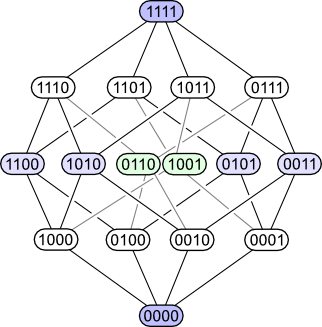
\includegraphics[scale=0.5]{hasse.png}
  \end{center}

  To perform OR, just do it digit by digit in hexadecimal form. For
  two hexadecimal digits, find the lowest common ancestor (LCA) and
  that would be the result. For AND just find LCA reversely.
  
  \begin{center}
    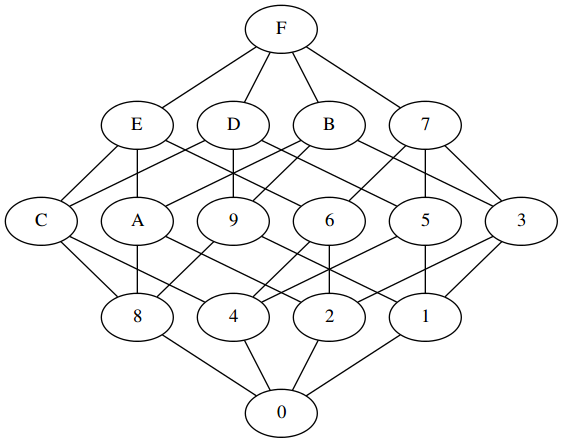
\includegraphics[scale=0.3]{hex_hasse.png}
  \end{center}

  Other logical operations can be replaced by AND, OR and NOT, where
  performing NOT we can simply find the centrosymmetric digit of each
  digit in the diagram above.

\item[2.52] See the table below.

  \begin{center}
  \begin{tabular}{l|c|c}
    \hline
    & x434F4D50 & x55544552 \\
    \hline
    Unsigned binary & 1129270608 & 1431586130 \\
    \hline
    1's complement & 1129270608 & 1431586130 \\
    \hline
    2's complement & 1129270608 & 1431586130 \\
    \hline
    IEEE 754 & 207.302001953125 & 1.4587137097728e13 \\
    \hline
    ASCII string & C0MP & UTER \\
    \hline
  \end{tabular}
  \end{center}

\item[2.56] It represents -18.0.
\end{enumerate}

\end{document}
